\documentclass[11pt, a4paper, german]{article}

\usepackage{booktabs}
\usepackage{algorithmic}
\usepackage[titlenotnumbered, vlined, ruled]{algorithm2e}
\usepackage{amsfonts}
\usepackage{amsmath}
\usepackage{amssymb}
\usepackage{amsthm}
\usepackage{mathtools}

\usepackage{array}
\usepackage[ngerman]{babel}
\usepackage[utf8]{inputenc}
\usepackage{color}
\usepackage{enumerate}
\usepackage{graphicx}
\usepackage{hyperref}
\usepackage{latexsym}
\usepackage{pdflscape}
\usepackage{makecell}
\usepackage{makeidx}
\usepackage{multirow}
\usepackage{pdfpages}
\usepackage{tikz}
\usepackage{tkz-fct}
\usepackage{tkz-graph}
\usetikzlibrary{patterns}
\usepackage{upgreek}
\usepackage{standalone}
\usepackage{slantsc}
\usepackage{lmodern}
\usepackage[labelformat=empty, font={scriptsize}]{subcaption}
\usepackage[labelformat=empty, font={scriptsize}]{caption}
\usepackage{pgfplots}
\usepackage{pgfplotstable}
\usepackage{circuitikz}
\usepackage{changepage}

\usetikzlibrary{shapes}
\usetikzlibrary{matrix, arrows,fit,shapes.gates.logic.US,shapes.gates.logic.IEC,calc,backgrounds,decorations.pathmorphing}




\DeclarePairedDelimiter\abs{\lvert}{\rvert}
\makeatletter
\let\oldabs\abs
\def\abs{\@ifstar{\oldabs}{\oldabs*}}
%
\let\oldnorm\norm
\def\norm{\@ifstar{\oldnorm}{\oldnorm*}}
\makeatother

\newcommand{\area}{\text{area}}
\newcommand{\uniquecone}{\text{unique\_cone}}
\newcommand{\uniquearea}{\text{unique\_area}}

\pgfplotsset{compat=1.8}

%
% Colors
%
\definecolor{darkblue}{RGB}{10, 0, 128}
\definecolor{grey}{RGB}{128, 128, 128}
\definecolor{darkred}{RGB}{180, 0, 0}
\definecolor{darkgreen}{RGB}{0, 100, 0}
\definecolor{lightgrey}{RGB}{210,210,210}
\newcommand{\RED}[1]{\textcolor{darkred}{#1}}
\newcommand{\BLUE}[1]{\textcolor{darkblue}{#1}}
\newcommand{\GREEN}[1]{\textcolor{darkgreen}{#1}}
\renewcommand{\emph}[1]{{\BLUE{#1}}}

\definecolor{darkRed}{rgb}{0.6,0,0}
\definecolor{lightRed}{rgb}{1,0.75,0.75}
\definecolor{darkGreen}{rgb}{0,0.5,0}
\definecolor{PineGreen}{rgb}{0.01,0.5,0.45}
\definecolor{darkBlue}{rgb}{0, 0, 0.75}
\definecolor{CornflowerBlue}{rgb}{0.15,0,0.7}
\definecolor{lightBlue}{rgb}{0.75,0.75,1}
\definecolor{grey}{rgb}{0.5,0.5,0.5}
\definecolor{black}{rgb}{0,0,0}
\definecolor{red}{rgb}{1,0,0}
\definecolor{green}{rgb}{0, 0.8, 0.3}
\definecolor{blue}{RGB}{10, 0, 128}
\definecolor{yellow}{rgb}{1,1,0}
\definecolor{orange}{rgb}{1,0.6,0}
\definecolor{cyan}{rgb}{0,0.7,1}
\definecolor{purple}{rgb}{0.5,0,0.8}

\newcommand\mycommfont[1]{\footnotesize\ttfamily\textcolor{darkGreen}{#1}}{}{}
\SetCommentSty{mycommfont}
\SetArgSty{textup}
\renewcommand\thempfootnote{\arabic{mpfootnote}}
\renewcommand{\thealgocf}{}

% \SetKwComment{Comment}{}{}

%
% Shorthands
%
\newcommand{\BL}{\textsc{BonnLogic}}
\newcommand{\Restr}{\textsc{And-Or}-Path Restructuring}
\newcommand{\AOP}{\textsc{And-Or}-Path}
\newcommand{\aop}{\textsc{And-Or}-path}

% \pgfpagesuselayout{resize to}[a4paper,landscape,border shrink=5mm]

% CONFIGURE PACKAGES

% NEW COMMANDS

\newcommand{\bl}[1]{\index{BonnLogic@\textsc{BonnLogic}!#1}}

\newcommand{\brent}[1]{\index{Brents adder@Brent's adder!#1}}

\newcommand{\ceil}[1]{\left\lceil #1 \right\rceil}

\newcommand{\delay}{\mathrm{delay}}

\newcommand{\depth}{\mathrm{depth}}

\newcommand{\floor}[1]{\left\lfloor #1 \right\rfloor}

\newcommand{\ld}{\log_{2}}

\newcommand{\loq}{\log_{\phi}}

\newcommand{\mini}[4]{\begin{minipage}{#1\linewidth}#3\end{minipage}\hfill\begin{minipage}{#2\linewidth}#4\end{minipage}}

\newcommand{\minialt}[4]{\centering{\begin{minipage}{#1\linewidth}#3\end{minipage}\begin{minipage}{#2\linewidth}#4\end{minipage}}}

\newcommand{\myindex}[1]{\emph{#1}\index{#1}}

\newcommand{\npfx}[1]{\index{non-prefix adders!#1}}

\newcommand{\OPT}{\mathrm{OPT}}

\newcommand{\pfx}[1]{\index{parallel prefix graph!#1}}

\newcommand{\size}{\mathrm{size}}

\newcommand{\sset}[1]{\left\{#1\right\}}

\newcommand{\todo}[1]{
  %\textcolor{red}{(TODO: \emph{#1})}
}

\newcommand{\vare}{\varepsilon}


% IMAGES

\newcommand{\tikzs}[2]{
  \centering
  \includegraphics[width=#1\linewidth]{images/#2.pdf} %fast
  %\ttikz{#2.tex}{#1} %slow
}
\newcommand{\tikzc}[3]{
  \centering{
    \includegraphics[width=#2\linewidth]{images/#3.pdf}
    \caption{#1}
    \label{fig:#3}%
  }
}
\newcommand{\tikzcc}[3]{
  \centering{
    \resizebox{#2\linewidth}{!}{
      \begin{tikzpicture}
        \input{images/#3}
      \end{tikzpicture}
    }
    \caption{#1}
    \label{fig:#3}%
  }
}
\newcommand{\ntikz}[1]{
  \begin{tikzpicture}
    \input{images/#1}
  \end{tikzpicture}
}
\newcommand{\ttikz}[2]{
  \centering{
    \resizebox{#2\linewidth}{!}{
      \begin{tikzpicture}
        \input{images/#1}
      \end{tikzpicture}
    }
  }
}
\newcommand{\ttikzfig}[3]{
  \begin{figure}[hbt]
    \centering{
      \resizebox{#2\linewidth}{!}{%
        \begin{tikzpicture}
          \input{images/#3}
        \end{tikzpicture}%
      }%
    }%
    \caption{#1}
  \end{figure}
}
\newcommand{\tikzfigs}[3]{
  \begin{figure}[hbt]%
    \centering{%
      \includegraphics[width=#2\linewidth]{images/#3.pdf}
      \caption{#1}%
      \label{fig:#3}%
    }%
  \end{figure}%
}
\newcommand{\tikzfigsc}[3]{
  \begin{figure}[hbt]%
    \centering{%
      \resizebox{#2\linewidth}{!}{%
        \begin{tikzpicture}
          \input{images/#3}
        \end{tikzpicture}%
      }%
      \caption{#1}%
      \label{fig:#3}%
    }%
  \end{figure}%
}
\newcommand{\tikzfig}[2]{
  \tikzfigs{#1}{1}{#2}
}


\usepackage{standalone}
\usepackage{slantsc}
\usepackage{lmodern}
%\newcounter{algorithm}
%\newtheorem{algorithm}[algorithm]{Algorithm}

\theoremstyle{plain}
\newtheorem{theorem}{Theorem}[section]
\newtheorem{cor}[theorem]{Corollary}
\newtheorem{lemma}[theorem]{Lemma}
\newtheorem{conj}[theorem]{Conjecture}
\theoremstyle{definition}
\newtheorem{definition}[theorem]{Definition}
\theoremstyle{remark}


\usepackage{caption}
\usepackage{subcaption}
\clubpenalty = 10000
\widowpenalty = 10000 
\displaywidowpenalty = 10000
\usepackage{Titelseite}
\usepackage{bbold}
\usepackage{graphicx}
\newcommand{\TM}{TechnologyMapping }

%Namen des Verfassers der Arbeit
\author{Alexander Zorn}
%Geburtsdatum des Verfassers
\geburtsdatum{26. Mai 1996}
%Gebortsort des Verfassers
\geburtsort{Bonn}
%Datum der Abgabe der Arbeit
\date{\today}

%Name des Betreuers
% z.B.: Prof. Dr. Peter Koepke
\betreuer{Betreuer: Prof. Dr. Stephan Held}
%Name des Instituts an dem der Betreuer der Arbeit tätig ist.
\zweitgutachter{Zweitgutachter: YYYY YYYY}
%z.B.: Mathematisches Institut
\institut{Forschungsinstitut f\"ur Diskrete Mathematik}
%Titel der Bachelorarbeit
\title{Heuristiken f\"ur das TechnologyMapping}
%Do not change!
\ausarbeitungstyp{Bachelorarbeit Mathematik}



\begin{document}

\maketitle

\tableofcontents
\newpage 
\section{Einleitung}

Der zunehmende Gebrauch elektronischer Geräte verlangt nach immer leistungsfähigeren Computerchips. Ein solcher wenige Quadratzentimeter große Chip beherbergt bis zu mehreren Milliarden Transistoren, welche, durch Drähte verbunden, gemeinsam eine Logische Funktion errechnen. Das Chipdesign beschreibt die Aufgabe aus einer gegeben Logischen Funktion einen herstellbaren Chip zu entwerfen, welcher diese Funktion realisiert. \\ 
\begin{wrapfigure}{r}{5.5cm}
	\scalebox{1}[-1]{
		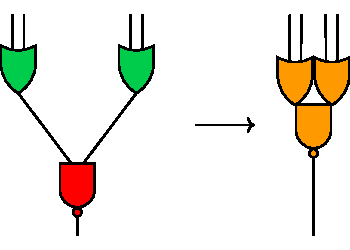
\includegraphics[]{pictures/compiled/einfBsp}
	}
		\caption{Zwei Realisierungen der Logischen Funktion $\neg((w\lor x) \land (y \lor z))$}
\end{wrapfigure}
Mithilfe von, aus wenigen Transistoren konstruierten, Bauteilen (genannt Gates, z.B.: AND, OR, INV, OAI) lässt sich eine Logische Funktion nachbilden. Abbildung 1 (links) zeigt dies an einem kleinen Beispiel.  Die Realisierung einer solchen Funktion ist jedoch nicht eindeutig, wie die in Abbildung 1 (links und rechts) gezeigte Nachbildung, beweist. \\
Die Größe der Menge aller möglicher Baupläne (später Circuit) für eine Logische Funktion hängt maßgeblich von der Anzahl der zur Verfügung stehenden Bauteile, sowie von dem Aufbau der Funktion, ab.
Es stellt sich heraus, dass im Allgemeinen eine Vielzahl möglicher Realisierungen einer Logischen Funktion existieren. Jedes Bauteil besitzt physikalische Eigenschaften an Größe, Geschwindigkeit (Delay) etc.. Somit besitzt auch jede Realisation solche Eigenschaften. \\
Ziel des \TM ist es für eine Logische Funktion eine Realisierung zu finden, welche eine Kostenfunktion (bestehend aus den physikalischen Eigenschaften) optimiert. Die Wahl der Implementierung hat direkte Auswirkungen auf die  Schnelligkeit, Größe und den Stromverbrauch des fertigen Chips. Hierbei geht das \TM von einer bereits realisierten Logischen Funktion aus und baut diese um zu einer möglichst kostengünstigen Alternative um. \\
Der optimale mögliche Umbau lässt sich bei kleinen oder eingeschränkten gegebenen Bauplänen noch in akzeptabler Zeit finden. Die Lösung dieses Problem für allgemeine Baupläne und Kostenfunktionen ist jedoch ein NP vollständiges Problem. Aus diesem Grund entwickelt die folgende Arbeit eine Heuristik, welche für sehr (mehrere 10.000 Bauteile) große Baupläne in akzeptabler Zeit einen möglichst kostengünstigen Umbau ermöglicht.
\newpage

\section{Terminologie \& grundlegender Algorithmus}
\subsection{grundlegende Definitionen}
Es folgen ein paar grundlegende Definitionen zur Beschreibung des Problems.

\begin{definition}{Boolesche Variable und Funktion: } \\
Eine boolesche Variable ist eine Variable mit Werten in $ \{ 0 , 1 \} $.
Sei $ n, m \in \mathbb{N}$. Eine boolesche Funktion ist eine Funktion $ f : \{ 0 , 1 \}^n \rightarrow \{ 0 , 1 \}^m $ mit n inputs und m outputs. 
\end{definition}

\begin{definition}{Gate und Library:}\\
Ein Gate $g$ mit Eingangsgrad $ n \in \mathbb{N}$ ist ein Tripel $(f_g, d_g, area_g)$. Hierbei sind $d_g, area_g \in \mathbb{R}_{\geq 0}$. Des Weiteren gilt $f_g$ ist eine boolesche Funktion mit $ f_g : \{0,1\}^n \rightarrow \{0, 1\} $. \\
Eine Library L ist eine Menge von Gates und sei $fanin_{max} := max\{ arity(g) | g \in L \}$.
\end{definition}
\begin{figure}[h]
\begin{center}
 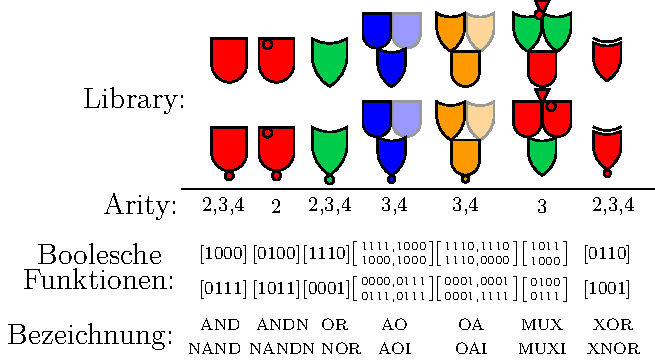
\includegraphics[height = 80pt]{./pictures/compiled/new_library.pdf}
 \caption{Beispiel einer Library}
 \label{fig:bsplib}
\end{center}
\end{figure}
$area_g$ gibt die Größe des physikalischen Bauteils an und $d_g$ beschreibt die Zeit die ein Signal braucht um von den inputs des Gates zu seinem Output zu gelangen. Dieser Wert lässt sich noch weiter differenzieren indem man $d_g \in \mathbb{R}^n$ wählt und somit Zeiten für jeden der Inputs angeben werden kann.\\

\begin{definition}{Circuit:}\\
Ein Circuit ist ein gerichteter kreisfeier Graph (directed acyclic graph DAG) mit folgenden Eigenschaften. Jeder Knoten gehört zu einer der aufgelisteten Kategorien: 
\begin{itemize}
\item{\bf Input} Knoten mit Eingangsgrad Null.
\item{\bf Gates} mit mindestens einer eingehenden Kante und ausgehenden Kante. Diese korrespondieren zu der Definition oben mit dem Zusatz dass an jedem der Inputs optional ein Inverter liegen kann.
\item{\bf Outputs} mit genau einer eingehenden Kante und keiner ausgehenden.
\end{itemize}
Ein Gate mit mehr als einer ausgehenden Kante wird auch Highfanoutgate genannt.\\
Ein Circuit realisiert durch Verschachtelung der booleschen Funktionen seiner Gates ebenfalls eine boolesche Funktion. \\
Zwei Circuits heißen äquivalent, wenn sie die gleiche boolesche Funktion realisieren.
\end{definition}

In einem Circuit lassen sich Teilgraphen durch ein Gate der Library austauschen. Voraussetzung für einen solchen Tausch ist, dass der veränderte Circuit äquivalent zu dem originalen ist. Dies sicher die folgenden Definitionen. 

\begin{definition}{Match und Kandidat:}\\
Sei g ein Gate in einem Circuit $C$. Ein (invertiertes) Match m ist ein Tupel $(p_m, I_m, f_m, inv_m)$ welches folgendes enthält:
\begin{itemize}
\item Ein Gate p der Library
\item Eine Menge X von Knoten aus der Circuit und eine Bijektion $ f: X \rightarrow inputs(p)$
\item Ein Funktion $ inv : inputs(p) \rightarrow \{not\_inv , inv \}$
\end{itemize}
So dass der Circuit $C'$, welcher durch den Austausch des Sub-Circuits von X bis g durch das Match (mit den durch inv definierten Invertern an den Inputs) entsteht, äquivalent zu C ist.
Ein invertiertes Match auf g ist ein Match auf g mit einem Inverter an jedem seiner Outputs.\\
Ein (invertierter) Kandidat auf g besteht aus einem (invertierten) Match auf g und einem Kandidaten für jeden Input Knoten von g (welcher kein Input von C ist).
\end{definition}

\begin{definition}{Circuit-Kandidat:}
Sei C ein Circuit mit Outputknoten Menge O. Eine Circuit-Kandidat K von C ist eine Menge von Kandidaten, sodass $\forall o \in O \, \exists!  h  \in K : h$ ist Kandidat von $ o$ und an jedem Knoten von C an dem sich mehrere Kandidaten überschneiden ist dasselbe Match gewählt.
\end{definition}
Folgendes Beispiel visualisiert die vorherigen Definitionen.\\
BILD EINSETZEN

Ein Circuit-Kandidat C ist eine Möglichkeit den Circuit physikalisch zu realisieren. Wie bereits in der Einleitung bemerkt gilt es nun den besten Kandidaten auf C auszuwählen. Dafür ist ein Maß für Implementierungen von Circuits notwendig. Es folgen zwei geläufige Beispiele. In der Praxis (und im späteren Verlauf dieser Arbeit) wird in der Regel eine convex-Kombination aus beiden verwendet.

\begin{definition}{Area und Delay eines Kandidaten:}\\
Sei C ein Circuit und K ein Circuit-Kandidat auf C. Dann gilt: \\
\begin{itemize}
\item $area(K) = \sum_{g \in gates(C)} (a_g + \sum_{i \in inputs(g)} \mathbb{1}_{\{inv_g(i)==inv\}} area_{inv})$ \\
wobei $area_{inv}$ die Größe eines Inverters ist.
\item $AT(K) = $\\$  \max\limits_{k \in can(K)} \{\max\limits_{i \in inputs(k)} \{   d_{gate(k)} + \mathbb{1}_{\{inv_g(i)==inv\}} d_{i} + AT(inp\_can(k,i)) + d_{w(k,i)} \} \}$ 
\end{itemize}
Wobei $can(K)$ die Menge der Kandidaten von $K$ sind und $inputs(k)$ sind die Inputknoten des Outputknoten des Kandidaten k. Des Weiteren ist $d_i$ das Delay eines Inverters und $d_{w(k,i)} $ das Delay der Kante zwischen den Knoten $k$ und $i$. $inp\_can(k,i)$ gibt den Kandidaten des $i$'ten Inputs von k zurück. 

\end{definition}

Das Delay (AT) gibt an wann das letzte Signal aus einem der Outputs des Circuit kommt.

\subsection{Kern Algorithmus}

Es folgt ein grundlegender Algorithmus, welcher auf eingeschränkten Circuits arbeitet, jedoch im weiteren Verlauf dieser Arbeit zu einer Heuristik für allgemeine sehr große Circuits erweitert wird.

\begin{problem}[framed]{(einfaches) Technology Mapping}
  Instanz:  & Circuit $C$ ohne Highfanoutknoten, mit eindeutigem Output $o$, Library $L$ mit beschr\"anktem $fanin_{max}$\\
  Aufgabe: &  Finde einen Kandidaten $K$ auf $o$, welcher die Arrivaltime/Area minimiert.
\end{problem}

\begin{algorithm}[H]
 \LinesNumbered
 \DontPrintSemicolon
 \caption{(einfaches) Technology Mapping}
 \SetKwInOut{Task}{Task}
 \KwIn{Circuit $C$ kreisfrei mit finalem Output $o$, Library $L$}

 bester\_kandidat[] $\gets \emptyset$\;
 bester\_inv\_kandidat[]$ \gets \emptyset$\;
 \ForEach{Knoten $v \in V(G)$ in topologischer Reihenfolge}
 {
   berechne alle (invertierten) Matches auf $v$\;
   \ForEach{ Match $m$ auf $v$ }
   {
      Berechne besten Kandidaten mit $m$ auf $v$\;
      Update best\_(inv)\_kandidaten\;
   }
 }
 Implementiere $C$ entsprechend bester\_kandidat[$o$]\;
\end{algorithm}\ \\

Dieser geht in topologischer Reihenfolge durch die Knoten v des Graphen und berechnet alle Matche auf v. Diese Matche werden dann zu einem Kandidaten ergänzt. Dieser Schritt (6) lässt sich sehr schnell implementieren, da für jedes Match m die besten Kandidaten der Inputs von m bereits bekannt sind.\\
 Ohne Highfanout-Knoten überschneiden sich diese nicht, und der beste Kandidat (inklusive der invertierten Verisonen) für jedes Match ist schnell gefunden. Von diesen wird der beste (in Bezug auf Area oder Arrivaltime) in Schritt 7 zu zur Liste der besten Kandidaten hinzugefügt.\\
 
\begin{cor}{Das (einfache) \TM besitzt \\ $\mathcal{O}(  |V(C)||L| fanin_{max})$-Laufzeit}\\
 	  Schritt 1 und 2 besitzen Laufzeit $\mathcal{O}(1)$. Schritt 4 lässt sich in \textcolor{red}{ wielange braucht es ein zu checken ob ein gate der Library ein Match eines Knoten sein kann ? ? plus Begründung! Laufzeit anpassen}. Schritt 6 ist wie bereits erwähnt schnell implementierbar, da für jeden der max $fanin_{max}$ Inputs der beste Kandidat verlinkt werden muss. Die Invertierten Matche werden nur gebarucht wenn der Input invertiert war. Somit braucht $\mathcal{O}(fanin_{max})$. Schritt 3 und 5 sind zwei verschachtelten Schleifen mit  $|V(C)|$ und max $|L|$ Durchläufen. \\
Daraus folgt eine Laufzeit von $\mathcal{O}(  |V(C)||L| fanin_{max})$. \hfill $\Box$
\end{cor}


\newpage
\section{Allgemeiner Algorithmus und Heuristik}
\subsection{Tradeoffprobleme}
Der oben vorgestellte Algorithmus ist in der Lage den bestmöglichen Umbau eines eingeschränkten Circuits zu bezüglich Area oder Delay zu errechnen. \\
Es existiert  ein Tradeoff zwischen beiden Area und Delay. Dies hat zur Folge, dass ein möglichst kleiner Circuit im Allgemeinen sehr langsam ist und man bei einer sehr schnellen Lösung mit einem großen Platzverbrauch rechnen muss. In der Anwendung des \TM ist jedoch weder ein sehr langsamer noch ein besonders grosser Circuit akzeptabel. Daraus folgt die Nachfrage nach einem Algorithmus, welcher in der Lage ist bezüglich einer Konvexkombination oder einer Schranke zu optimieren. Daraus ergeben sich die beiden folgenden Optimierungs-Probleme: \\
\textcolor{red}{Hier beide Probleme einfügen}\\


Diese \textcolor{red}{diese Probleme sind äquvalent Beweis? oder verweis aus quelle}

Dadurch ergibt sich folgende Problemstellung für den Algorithmus: An jedem Knoten v lässt sich jetzt nicht mehr nur der Kandidat speichern, welche die Kostenfunktion an v optimiert. Angenommen v liegt in einem sehr Delay kritischen Gebiet des Graphen, dann kann es sehr gut sein dass es für einen Nachfolger von v sehr günstig ist v vollständig auf Delay hin zu optimieren und seine Kosten zu verbessern, was jedoch nicht möglich ist wenn der einzige an v gespeicherte Kandidat dieser ist der die Kosten ( Konvexkombination) an optimiert. \textcolor{red}{diesen satz verbessern!}\\
Die Kosten eines Kandidaten k sind somit nicht $\lambda AT(k) +(1-\lambda )area(k)$,  sondern das Tupel $(AT(k), area(k))$.
Es gibt jedoch eine Klasse von Kandidaten, welche nicht gespeichert muss. Dazu folgende Definition\\

\begin{definition}{(dominierte Kandidaten)}\\
	Seien $k_1, k_2$ Kandidaten desselben Knotens. Dann wird $k_1$ von $k_2$ dominiert, wenn gilt:\\
	$AT(k_1) < AT(k_2) und area(k_1) \leq area(k_2)$\\
	$	AT(k_1) \leq AT(k_2) und area(k_1) < area(k_2)$\\	
\end{definition}

Eine optimale Lösung des \TM verwendet offenbar (\textcolor{red}{in einem Korollar beweisen ?}) nur nicht-dominierte Kandidaten, woraus folgt, dass nur diese während der Ausführung des Algorithmus gespeichert werden müssen.\\
Die Menge der noch bleibenden Kandidaten lassen sich in sogenannten Tradeoff-Kurven speichern (siehe Abbildung ?? \textcolor{red}{Abbildung hinzufügen.. kann ich Lucas verwenden ?}). Welche jeden Kandidaten zweidimensional anhand seiner Kosten erfasst.


\textcolor{red}{Next things todo: Algorithmus erweitern und dann auf die Filterung mit Buckets eingehen inclusive der funktionierenden epsilon betrachtung -> ohne beweis mit erklärung}

ZSFG:

1. Vorstellung der Probleme: die da wären :

	-Tradeoffprobleme -> mehrere Kandidaten müssen gespeichert werden. Einführung der Tradeoff Kurven und Bucket Filterungen (wir sind noch in Bäumen dies lässt sich also noch in den Alg einbauen und beweisen) 
	
	-Highfanoutgates -> Einführung von Klassen widerrum erweitern des TM algos 
	
	=> bei konstantem k gibt es zu diesem Punkt noch einen FPTAS -> besonder hilfreich auf schlechteste Wege pfade kann auch erst später erwähnung finden
	
	-required ATs einführen und sagen dass sie aktuell noch äquivalent sind 
	
	-multiple outputs -> sagen, dass optimieren auf AT nicht mehr Funktioniert da es nicht nur eine AT gibt. man könnten die latest AT verbessern, das ist jedoch nicht das was man möchte. neue Kosten optimierung mit RAts definieren. Des weiteren nicht vergessen, dass über outputs nicht gemacht werden darf 
	
	-reduandant gates -> soll das hier hin ? 
	
	=> Algorithmus verallgemeiner und erste Heuristik bauen, welche auf Area  und RATs hin optimiert

\section{Präprozessing  zusätliche Addons}
	-auseinanderbauen von gates : Beispiele und einegehen auf vor und nachteile genauerer bezug in der Laufzeitanalyse
	
	-errechnen kleiner optimal gelöster häufig vorkommender Instanzen -> unabh. von dem auseinanderbauen.  -> lässt sich beweisen dass eine auseinandergebaute instanz sich in das bestmögliche Machting matchen lässt ? 
	

\section{Weitere Optimierungskriterien}
	-Vt Optimierung -> Optimierung bezüglich Power
	
	-Layer assignment -> sehr kurz und grobe übersicht kommt später noch auf die TODOs 
	
	
\section{Version der Heuristik, welche obige Kriterien beherzigt}

\section{Laufzeitanalyse}

\section{Fazit und Ausblick}
	







\newpage
%\clearpage

\end{document}
